%%%%%%%%%%%%%%%%%%%%%%%%%%%%%%%%%%%%%%%%%
% Seismica preamble + title block for the Cascadia catalog paper.
%
% This is the STABLE "shell head". It is prepended to the Quarto-rendered body
% (paper/main.qmd -> body) by paper/build.py to assemble the full paper/main.tex.
% Edit AUTHORS / AFFILIATIONS / CREDIT here (they change rarely); the TITLE,
% SHORTTITLE, REPORTTYPE and ABSTRACT come from main.qmd's front matter (the
% %%...%% placeholders below are substituted by build.py). Edit the PAPER BODY
% in paper/main.qmd.
%%%%%%%%%%%%%%%%%%%%%%%%%%%%%%%%%%%%%%%%%

%% Options: anonymous | breakmath | languages | preprint | report | review
\documentclass[review]{seismica}
% NOTE: the original Overleaf preamble loaded BOTH subfig and subcaption, which
% are mutually incompatible; keep only subcaption (compatible with the class's
% caption package) for any multi-panel figures.
\usepackage{subcaption}

\title{A Unified Deep-Learning Pipeline for Cascadia Earthquake Cataloging}
\shorttitle{Ensemble Cascadia}
\reporttype{Fast Report}

\author[1]{Marine~Denolle
\orcid{0000-0002-1610-2250}
\thanks{Corresponding author: mdenolle@uw.edu}
}
\author[1]{Hiroto Bito
\orcid{0009-0001-4138-0287}
}
\author[1]{Qibin~Shi
\orcid{2222-2222-2222-2222}
}
\author[1]{Yiyu~Ni
\orcid{3333-3333-3333-3333}
}
\author[2]{Ian W. McBrearty
\orcid{3333-3333-3333-3333}
}
\author[3]{Zoe~Krauss
\orcid{3333-3333-3333-3333}
}
\author[4]{Nathan T. Stevens
\orcid{0000-0001-5648-2254}
}
\author[2]{Yifan Yu
\orcid{0000-0001-5986-9702}
}
\author[2]{Gregory C.~Beroza
\orcid{3333-3333-3333-3333}
}

\affil[1]{Department of Earth and Space Sciences, University of Washington, Seattle, USA}
\affil[2]{Department of Geophysics, Stanford University, USA}
\affil[3]{School of Oceanography, University of Washington, Seattle, USA}
\affil[4]{Pacific Northwest Seismic Network, University of Washington, Seattle, USA}

% --- pandoc/Quarto body helper macros -------------------------------------
% The body is produced by pandoc (via quarto) and may use these helpers, which
% normally live in Quarto's own preamble (replaced here by this Seismica head).
% Defined defensively so the assembled main.tex compiles standalone.
\providecommand{\tightlist}{\setlength{\itemsep}{0pt}\setlength{\parskip}{0pt}}
\providecommand{\passthrough}[1]{#1}
\providecommand{\pandocbounded}[1]{#1}
\graphicspath{{figures/}{./}}
% Network DOIs in the .bib contain underscores (e.g. 10.7914/SN/7D_2011); outside
% math an underscore triggers "Missing $". Detokenize the printed DOI (hyperref
% handles the underscore in the URL argument), keeping the reference hyperlinked.
\AtBeginDocument{\renewcommand{\doi}[1]{\href{https://doi.org/#1}{doi:\detokenize{#1}}}}

%% Author CRediT roles (https://casrai.org/credit)
\credit{Conceptualization}{Name Firstauthor, Name Thirdauthor}
\credit{Formal Analysis}{Name Firstauthor, Name Secondauthor}
\credit{Writing - Original draft}{Name Firstauthor}

\begin{document}

\makeseistitle{
    \begin{summary}{Abstract}
blablba
    \end{summary}
}


\section{Introduction}\label{introduction}

\subsection{Coastal and Offshore Pacific
Northwest}\label{coastal-and-offshore-pacific-northwest}

The Pacific Northwest hosts a complex and geologically diverse plate
boundary system. The young and buoyant Juan de Fuca (JdF) Plate is
generated at the Juan de Fuca Ridge and is subducting beneath the North
American Plate along the Cascadia Subduction Zone (CSZ) at a rate of
30--45~mm~yr\(^{-1}\) \citep[e.g.,][]{McCaffrey07}. The JdF Plate is
bounded to the North by the Nootka and Explorer transform systems and to
the South by the Gorda and Mendocino fracture zones, forming a narrow
oceanic plate undergoing deformation along multiple styles of plate
boundaries. The CSZ extends roughly 1,100~km from Vancouver Island,
British Columbia, to northern California, encompassing both subduction
and strike-slip fault systems that accommodate deformation between the
JdF, Gorda, and North American plates \citep{Wang16, Walton21}. Despite
the clear evidence from paleoseismic and tsunami deposits for repeated
\(M\)~8--9 megathrust earthquakes every 250--500~years
\citep[e.g.,][]{Atwater92, Nelson21}, the subduction interface exhibits
remarkably low background seismicity compared to other subduction zones
worldwide since the instrumental record. This contrast between low
interseismic activity and high geologic hazard is commonly attributed to
strong, spatially variable coupling on the megathrust and the
sediment-rich nature of the incoming plate, which together may suppress
small-scale brittle failure \citep{Hyndman93, Walton21}. Understanding
this quiescence and its spatial heterogeneity remains a fundamental
challenge for constraining future megathrust rupture potential in
Cascadia.

Monitoring this offshore subduction zone is intrinsically difficult due
to the logistical and technical challenges of maintaining ocean-bottom
sensors in deep water. The onshore networks that form the backbone of
regional earthquake early warning systems---operated by the Pacific
Northwest Seismic Network (PNSN), the Northern California Earthquake
Data Center (NCEDC), and Natural Resources Canada---are confined to the
continental margin and have limited sensitivity to offshore events.
Their detectability is further reduced by unfavorable network geometry
and the pervasive coastal microseism noise that often masks tectonic
signals \citep[e.g.,][]{Webb98}. To extend offshore coverage, research
observatories such as the Ocean Networks Canada (NEPTUNE) and the Ocean
Observatories Initiative (OOI) Regional Cabled Array provide continuous
but spatially sparse records focused on specific features like the Axial
Seamount and Hydrate Ridge. A key advance came from the community-led
Cascadia Initiative (CI) experiment \citep{Toomey14}, which from
2010--2015 deployed a rolling array of more than 70 ocean bottom
seismometers (OBS), represented in
Figure~\hyperref[fig:fig1]{{[}fig:fig1{]}}, spanning the full width of
the subduction system---from the outer Pacific Plate, across the trench,
to the forearc and coast, and from the Nootka Fault in the north to the
Mendocino Triple Junction in the south. This experiment yielded an
unprecedented, five-year plate-scale dataset for characterizing
seismicity (REF), structure (REF), and fault-zone behavior offshore
Cascadia (REF).

Although the CI network transformed offshore seismic monitoring, high
oceanic noise levels and sparse coverage still limited the detection of
small earthquakes \citep{Stone18, Morton23}. Initial analyses using
traditional short-term average-to-long-term average (STA/LTA) detection
identified a few hundred new events along the subduction interface and
in the overriding plate \citep{Stone18}. Building on this foundation,
\citeauthor{Morton18} \citetext{\citeyear{Morton18}; \citealp{Morton23}}
applied template matching and subspace detection to continuous CI data
with a focus on the CSZ, combining land and OBS networks to reveal over
4,000 previously undetected events, particularly concentrated near
subducted seamounts at \ensuremath{\sim}44°N and along the downdip edge
of the seismogenic zone beneath Vancouver Island (see Figure
\hyperref[fig:fig1]{{[}fig:fig1{]}}). These results established that
small-magnitude earthquakes preferentially occur near asperity
boundaries or downdip transition zones rather than within strongly
locked regions. While interplate seismicity in the CSZ remains sparse,
the surrounding plate boundaries are far more active: the Mendocino
Triple Junction produces frequent \(M\)~5--7 strike-slip and intraplate
events on the Gorda Plate (REF), the Blanco Fracture Zone \citep{Liu25}
regularly hosts large transform earthquakes (e.g., the 2021 \(M\)~6.9
event), and to the north, the Nootka Fault accommodates complex
intraplate deformation between the JdF and Explorer Plates with
earthquakes up to \(M\)~6.5 (REF). Together, these surrounding sources
of seismicity highlight the tectonic vigor of the Cascadia margin and
underscore the need for comprehensive, plate-scale analyses capable of
linking offshore microseismicity with regional deformation processes.

\begin{figure}
\centering
\includegraphics[width=\linewidth]{figures/fig1.png}
\caption{Network of Stations and Benchmark Earthquake Catalogs: (a) Map of all
seismic stations, color-coded by the number of days they were active, used, and
(b) benchmark earthquake catalogs from ANSS (green) and Morton-2023 (yellow)
\citep{Morton23}.}
\label{fig:fig1}
\end{figure}

\subsection{Earthquake Catalog
Building}\label{earthquake-catalog-building}

Recent advances in machine learning have revolutionized the way
seismologists construct earthquake catalogs. Deep learning enables
automated detection of weak and overlapping seismic signals buried in
noise, producing catalogs that are far more complete and higher in
spatial--temporal resolution than those derived from traditional
algorithms \citep{poggiali2025fault, mousavi2023machine}. The typical
modern workflow consists of three key steps: (1) phase detection and
picking, (2) phase association, and (3) event location and relocation
\citep[e.g.,][]{zhu2022endtoend, zhu2023quakeflow, Isken25, Shiddiqi25}.

\subsection{Detection and Phase
Picking}\label{detection-and-phase-picking}

Recent years have seen rapid advances in deep learning architectures for
seismic phase detection and picking, ranging from simple regression
networks such as the Generalized Phase Detection (GPD) model
\citep{ross2018generalized} and U-Net architectures like \emph{PhaseNet}
\citep{zhu2019phasenet}, to more complex encoder--decoder models such as
the \emph{EQTransformer} \citep{mousavi2020earthquake}. These models
learn directly from waveform data to identify P- and S-arrivals and have
produced denser catalogs that capture weak, overlapping events, greatly
improving catalog completeness compared to conventional algorithms
\citep{mousavi2023machine, zhu2022endtoend}. However, models originally
trained on continental datasets show substantially reduced performance
when applied to ocean-bottom seismometer (OBS) recordings due to
coupling differences, reverberations, and complex noise structures
\citep{ruppert2022}. To address this challenge, recent developments have
focused on retraining and adapting pickers for marine environments. Two
state-of-the-art examples, both implemented within the open-source
\emph{SeisBench} framework \citep{woollam2022seisbench}, are
\emph{OBSTransformer} and \emph{PickBlue}. \emph{OBSTransformer}
\citep{niksejel2024obstransformer} leverages automated labeling,
transfer learning from land data, and a transformer-based encoder to
improve generalization to noisy offshore waveforms, achieving higher
recall and precision across distances. \emph{PickBlue}
\citep{bornstein2024pickblue} extends EQTransformer and PhaseNet by
adding a hydrophone channel and retraining on a global OBS dataset
comprising 15 deployments and over 13,000 events, significantly
enhancing phase onset accuracy. While these specialized models show
superior performance for specific data types, ensemble deep learning
remains the most robust and generalizable strategy for heterogeneous
networks. By aggregating probability fields from multiple pretrained
pickers such as PhaseNet, EQTransformer, and GPD, ensemble frameworks
achieve improved recall and precision without retraining, demonstrating
excellent performance across land, OBS, and distributed acoustic sensing
(DAS) data \citep{yuan2023, shi2025, gaete2025}. Although
computationally demanding, ensemble methods offer consistent performance
across sensor types and are well-suited for on-premise or
high-performance computing workflows. Once P and S arrivals are
identified from continuous waveforms, these phase picks must be
associated with coherent earthquake events to construct the catalog.

\subsection{Phase Association}\label{phase-association}

Recent developments in phase association algorithms have greatly
improved the scalability of earthquake cataloging workflows to dense
seismic networks and high pick rates. Classical grid- and model-based
approaches such as \emph{REAL} and \emph{GaMMA} remain computationally
efficient for regional datasets, but their performance declines under
high-noise or high-density conditions. Newer algorithms such as
\emph{PyOcto} and the graph neural network-based \emph{GENIE} achieve
near-perfect association accuracy in both crustal and subduction
environments while maintaining strong scalability to large or
heterogeneous networks \citep{Puente2025}. Benchmarking studies
demonstrate that these methods outperform earlier associators,
particularly in scenarios involving overlapping events or variable
network geometry. Because GENIE learns spatial and temporal
relationships directly from data and can adapt to varying network
configurations, it is particularly well suited to the hybrid land--ocean
seismic networks of Cascadia, where heterogeneous station coverage and
complex wave propagation challenge traditional association schemes.

\subsection{Challenges and Opportunities in
Cascadia}\label{challenges-and-opportunities-in-cascadia}

Given the vast extent of the JdF plate and its complex tectonic features
at the various boundaries, most high-resolution earthquake catalogs have
so far targeted specific smaller regions. The Axial Seamount has been
extensively studied for its magmatic and volcanic activity
\citep[e.g.,][]{Wilcock2016, Waldhauser2020}, while the Endeavor segment
has received attention for its diking events and hydrothermal
circulation \citep[e.g.,][]{Krauss2019}. Temporary arrays have been
deployed along the Nootka fault zone to capture transform and intraplate
seismicity, and multiple amphibious experiments have been conducted near
the Mendocino Triple Junction to study the interactions among the Gorda,
Pacific, and North American plates \citep[e.g.,][]{Yoon2024}. More
recently, efforts have revisited Cascadia Initiative (CI) data using
modern machine learning tools, deep learning pickers applied to the
Blanco Transform Fault \citep{liu25} and Axial Seamount \citep{wang},
revealing substantial improvements in catalog completeness. However,
these studies remain localized and methodologically heterogeneous,
lacking a unified framework that can consistently capture seismicity
across the entire Juan de Fuca system.

This work addresses this gap by implementing a holistic workflow that
combines ensemble deep learning phase pickers, scalable association
using the \emph{GENIE} graph neural network, and relocation through both
double-difference methods (\emph{GraphDD}) and cross-correlation-based
differential times. This integrated approach enables the construction of
a consistent, high-precision catalog spanning the diverse tectonic
environments of Cascadia. The manuscript is organized as follows:
Section~\ref{sec:data} describes the datasets, from waveforms to
baseline catalogs, used; Section~\ref{sec:methods} details the catalog
building pipeline and quality control measures;
Section~\ref{sec:results} presents the resulting earthquake catalogs and
comparisons with baseline catalogs; and Section~\ref{sec:disc} discusses
the tectonic and methodological implications of these results. We
conclude with recommendations for future improvements and extensions of
this framework to real-time seismic monitoring in Cascadia.

\section{Data}\label{sec:data}

\subsection{Baseline Earthquake
Catalogs}\label{baseline-earthquake-catalogs}

To establish a reference for comparison, we compile two baseline
earthquake catalogs that represent the state of regional seismic
monitoring prior to the application of modern deep learning workflows.
The first catalog is the Advanced National Seismic System (ANSS)
catalog, maintained by the U.S.~Geological Survey. This catalog is based
on detections from permanent onshore seismic stations and serves as the
authoritative record for regional seismicity. Prior to the expansion of
real-time earthquake early warning capabilities in the Pacific
Northwest, the density of operational stations in Oregon and Washington
was sparse relative to present-day coverage, limiting the completeness
of the regional catalog. For this study, we extracted ANSS events
between 38°--51° N and 119°--132° W, spanning 1 January 2011 to 31
December 2015 UTC. The resulting distribution shows that most recorded
events during this period cluster in Washington State and near the
Mendocino Triple Junction (Figure \hyperref[fig:1]{{[}fig:1{]}}b),
reflecting the higher station density in those regions.

We also include the high-resolution earthquake catalog from
\citet{Morton23}, who applied a subspace detection approach that used
STA/LTA-detected template events from \citet{Stone18} to define signal
eigenmodes and conduct subspace detection across the four-year
deployment. Their catalog focuses on the Cascadia Subduction Zone,
encompassing the Juan de Fuca and Gorda plates between approximately 39°
N and 49° N, and reports tens of thousands of low-magnitude events that
were previously undetected in regional catalogs. The newly detected
seismicity highlights several key zones of activity: the Mendocino
Triple Junction and adjacent Gorda plate, central Cascadia, where
seamounts subduct beneath the margin, and the region west of Vancouver
Island---likely representing activity downdip of the seismogenic zone
and updip of the slow-slip region (Figure
\hyperref[fig:fig1]{{[}fig:fig1{]}}b). Together, we label \texttt{ANSS}
and \texttt{Morton23} the two catalogs \citet{Morton23} that provide a
robust baseline for assessing the improvement in detection and location
capabilities afforded by deep learning--based cataloging workflows.

\subsection{Waveform Data}\label{waveform-data}

Waveform data were retrieved using \emph{ROVER}, an EarthScope
Consortium product designed for large-scale, programmatic waveform data
access and management. We collected all available continuous seismic
data between 2010 and 2015 from stations within a broad region
encompassing the CSZ and its surrounding tectonic boundaries. The
dataset includes OBS records from the CI experiment \citep{Stone2018},
along with permanent and temporary land-based stations operated by
regional networks across Washington, Oregon, and Northern California.
The CI experiment deployed over 100 OBS instruments across four yearly
cruises between 2010 and 2015, complemented by more than 60 coastal and
nearshore broadband stations. After inspecting metadata, gain, and
timing consistency, we identified \texttt{XX} CI OBS and \texttt{XX}
onshore stations with continuous, high-quality recordings suitable for
analysis.

The station data were initially gathered from the region bounded by
123°--127°W and 40°--50°N. During early testing, we found that this
spatial window limited the number of peripheral stations available for
constraining event locations and verifying phase association. To improve
azimuthal coverage and increase the robustness of association and
relocation, we expanded the domain to include stations from 122°--123°W
onshore and 127°--129°W offshore. This iterative approach ensured
sufficient network geometry to resolve offshore and intraslab events.
The following seismic networks were included: \texttt{C8}, \texttt{7D},
\texttt{7A}, \texttt{CN}, \texttt{NV}, \texttt{UW}, \texttt{UO},
\texttt{NC}, \texttt{BK}, \texttt{TA}, \texttt{OO}, \texttt{PB},
\texttt{X6}, \texttt{Z5}, and \texttt{X9}. Three-component data were
used for ensemble phase picking. When both \texttt{BH} and \texttt{HH}
channels were available, only the higher-bandwidth \texttt{HH} channels
were retained. However, to increase land-based coverage, the workflow
was later extended to include \texttt{EH} channels, which improved
spatial sampling along the margin without compromising signal fidelity.

Waveform preprocessing followed the data conditioning pipeline typical
of the deep learning phase picking \emph{EQTransformer}
\citep{mousavi2020earthquake}. Each continuous waveform was bandpass
filtered between 4--15~Hz to remove low-frequency microseismic noise,
following the processing strategy of \citet{Morton2023}, who
demonstrated improved detectability of small-magnitude events above 4~Hz
in Cascadia OBS data. Short data gaps were filled by linear
interpolation using the \texttt{ObsPy} \texttt{Stream.interpolate()}
method, and all traces were resampled to 100~Hz to match the input
sampling rate required by the deep learning models.

In total, the dataset comprised approximately 582,936 station-days of
continuous three-component data, corresponding to about 56~TB of
waveform data after preprocessing. All processing and metadata
management steps were scripted to ensure reproducibility and
traceability of data provenance.

\subsubsection{Known Data Issues}\label{known-data-issues}

Background oceanic noise in the same frequency band as regional
earthquakes (5-12 Hz) tends to be higher for shallower CI stations on
the continental shelf, where noise from ocean waves dominates
\citep{hilmo_wilcock_2020}. Noise from passing ships can also dominate
regional earthquake frequencies on Cascadia OBS \citep{krauss25}; the
northwest Pacific basin is a major shipping corridor
\citep{dahl_trends_2021}.

Various marine-specific impulsive noise signals, which most ML pickers
are not trained to recognize as non-earthquakes, are present on CI OBS.
Most CI stations have also been shown to record short-duration events
(SDEs), which are impulsive single-phase arrivals lasting \textless{} 5
s \citep{hilmo_wilcock_2020, macleod_nonseismic_2025}. SDEs are inferred
to be non-tectonic and are observed on OBS globally, typically on only
one OBS at a time. Likely source mechanisms include biological sources
such as ``fish bumps'' or gas-related sources such as bubbles moving
through sediment \citep{batsi_nonseismic_2019, tary_atypical_2024}.
\citet{MacLeod25} found that SDEs on the CI stations likely have a mix
of biological and physical mechanisms. Shallower CI stations on the
continental shelf at depths \textless{} 1000 m tend to record more of
these SDEs, with rates of \textgreater{} 2000 per day for some of the
shallowest instruments. T-phases, which are tertiary earthquake arrivals
that travel through the ocean as acoustic phases, also occur frequently
in the northwest Pacific basin due to the proximity to active mid-ocean
ridges and transform faults
\citep{dziak_20-year_2011, shen_ocean_2024, liu_automatic_2025, krauss25}.
Depending on relative source and receiver depths, T-phases are often
more strongly recorded than body wave arrivals such as P- and S-waves,
and are sometimes the only earthquake arrival recorded for regional
earthquakes by OBS on the Cascadia margin \citep{krauss25}.

Consultation of the CI data report \citep{obsic2011cascadia} In
consultation with the CI data report (REF5), phase picking data from sta

First, we pick on day-long mseed files, we store the data into CSV
files, and run this embarrassing parallel using Dask.els

\section{Methods}\label{sec:methods}

\subsection{ML Pipeline}\label{ml-pipeline}

\subsubsection{Phase Picking}\label{phase-picking}

The process is multi-stage. First we pick on day-long mseed files, we
store the data into CSV files and run this embarassing parallel using
dask. Second

\begin{figure}
    \centering
    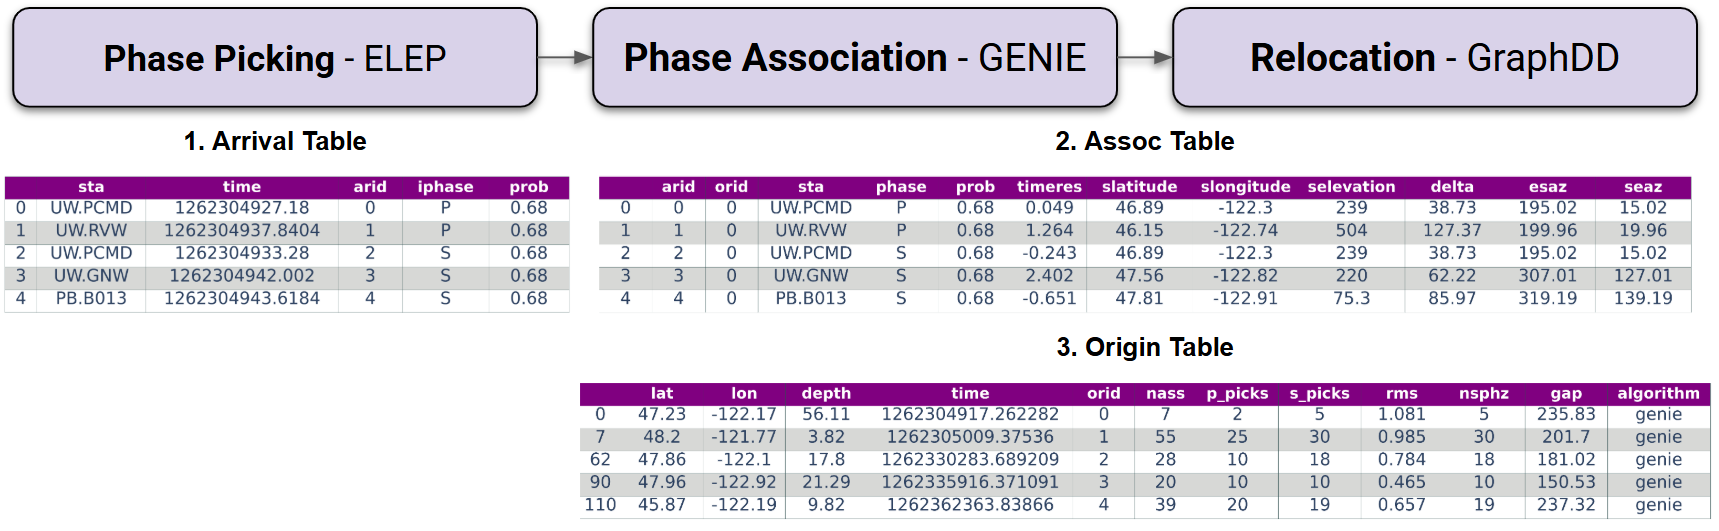
\includegraphics[width=\linewidth]{figures/fig2.png}
    \caption{Earthquake Catalog Pipeline.}
    \label{fig:fig2}
\end{figure}

There are three methods for the prediction by semblance: statistical,
coherent, and learning approaches. The statistical-based semblance will
take the maximum probabilities among multiple predictions and keep it
for the P- or S-phase. The coherence-based ensemble will output the
probabilities in time series by applying a certain semblance
calculation. The \textbf{phase picking} by ensemble learning was run
from the first day of the year to the last day of the year from 2010 to
2015 (Yuan et al., 2023).

For the EQTransformer, the original model, ETHZ, INSTANCE, SCEDC, and
STEAD were used. The picking threshold was set to 0.05 for both P and S
picks(Yuan et al., 2023). The P and S picks for each station for each
day were saved in a CSV file in the Seisbench format. data is normalized
to min-max for teh ETH, INSTANCE, SCEDC, STEAD. pretrain\_list =
{[}`original', `ethz', `instance', `scedc', `stead'{]}

\subsubsection{Training PINN for travel
time}\label{training-pinn-for-travel-time}

Accurately modeling seismic travel times through arbitrary velocity
models is a key step of all earthquake detection and location workflows.
Many works rely on established frameworks such as ray tracing for
layered media {[}TauP and NonLinLoc{]} or the fast-marching method
{[}{]} for first-arrival times in 3D velocity models.

To increase the efficiency of training and implementing GENIE and
GraphDD, we train a 3D PINN neural network surrogate travel time
calculator {[}Smith, Anderson{]}, using the codes of {[}GENIE{]}. This
mitigates the need to store large and expensive travel time tables in
memory, and also makes the travel times automatically differentiable,
which is required for training GraphDD. To increase the accuracy of this
PINN and achieve stable training, the model uses the hybrid
velocity-and-travel time estimation approach introduced in {[}{]}, as
well as the sinusoid activation function {[}{]} to improve stability of
differentiation and representation of high-frequency structure. The
3-layer FCN model (\ensuremath{\sim} free parameters) representing the
travel time surrogate is trained with a combination of both the
physics-informed eikonal equation (PDE) and real-data losses, using the
fast-marching method {[}{]} implemented in as ground truth.

The model is trained to emulate the full-waveform derived 3D velocity
model of {[}{]}, which used long-period teleseismic waves to constrain
the P and S wave velocity structure of the upper mantle and crust of
much of the western USA. Due to it's depth sensitivity, this model has
largely high velocities even at shallow depths, which is suitable for
the offshore basaltic rheology domains {[}{]}, however leads to
over-estimates of velocity for on-shore seismicity. Nevertheless we use
this velocity model for it's expansive 3D coverage and respecting of the
overall tectonic structure of the region (Fig. SX). The fitted PINN has
an average RMS residual of X s, corresponding to a X relative error
compared to the ground-truth fast marching method simulations (Fig. SX).

\subsubsection{Association}\label{association}

We train a regional version of GENIE for Cascadia spanning 38˚N to 51˚N
and 119˚W to 132˚W, and including all available seismic and OBS stations
during our study (Fig. X). This typically ranges from \ensuremath{\sim}
to \ensuremath{\sim} stations a day. To train the model, we simulate
travel times using the 3D model of (Arthur Rodgers et al., unpublished),
and generate a wide variety of synthetic earthquake sources spanning
different source regions, maximum moveout distances of phases, event and
noise rates, and the number of monitoring stations from within the full
network. This allows the model to specialize in the conditions of the
Cascadia subduction zone while also handling the diversity of seismicity
(and available station sets) that may occur during the study.

Once trained, we apply the model to each day of available seismic data,
using the subset of available stations on each day to construct the
station graphs. Such station graphs can vary widely in spatial coverage
due to differences in the availability of OBS stations (e.g., Fig. SX).
We apply the model with fixed detection and association thresholds of
0.5 to all days, and then locate all events using the associated picks
with least squares minimization \citep{lomax2000probabilistic}. We only
keep events with at least five stations with associated picks. This
provides the initial catalog of earthquake source locations, origin
times, and phase associations. This includes \ensuremath{\sim} sources,
and \ensuremath{\sim} associated P and S waves, with an average rate of
\ensuremath{\sim} events per day.

\subsubsection{Waveform coherence}\label{waveform-coherence}

We formed candidate event pairs by selecting events with preliminary
locations within \(0.1^\circ\) of each other, yielding
\ensuremath{\sim}52 million pairs considering EH, BH, and HH stations.
For each arrival, we extracted waveform windows from 1~s before to 2~s
after the pick and estimated differential travel times and waveform
coherence in the 1--10~Hz band using moving‑window cross‑spectral
analysis (MWCS; \citep{poupinet_monitoring_1984}). MWCS results were
averaged across three channels. We retained measurements with coherence
\(>0.1\), resulting in \ensuremath{\sim}56 million differential
travel‑time observations. This double‑difference data set was then used
to relocate events with GraphDD.

\subsubsection{Relocation}\label{relocation}

We re-locate the initial GENIE catalog using the GraphDD relocation
model \citep{mcbrearty2024double}. This deep learning double-difference
relocation method is effective for large-scale catalogs and is based on
a similar graph neural network architecture as GENIE. For this step, we
first remove isolated events with fewer than 10 neighbors within 10 km,
then construct a large dataset of source-station `double-difference'
input graphs, which capture features related to the double-difference
residuals, the initial source locations, and the relative source and
station distributions. GraphDD is then trained to directly minimize the
standard double-difference residual loss function {[}{]} by estimating
source relocation values. Upon convergence, the double-difference
residuals of the catalog have been substantially minimized (Fig. SX),
and the relative resolution of earthquake locations has been enhanced
(Fig. SX), as expected from double-difference methods. This relocated
catalog has 63,887 events and highlights major expected tectonic
features, such as {[}{]}, as well as local quaries and volcanoes (Fig.
SX). This catalog is further analyzed and quality-controlled in the
following sections.

\subsubsection{Alternative pipeline
tested}\label{alternative-pipeline-tested}

we tested the pyocto + hypoinverse by running pyocto in individual
velocity model, then merged the events. Location artifacts. refinemenent
with hypoinverse. why we gave up.

Association was performed using PyOcto (Munchmeyer 2024) on each of the
subsets, such that only picks made on stations within the same subregion
could be associated into events. However, the associator was allowed to
locate events over the entire study area, assuming the subregion 1-D
velocity model everywhere. The associator required at least 1 P pick and
3 S picks for an event. The PyOcto association outputs two dataframes,
the data frame for the associated events and one in which each pick
information is assigned to the corresponding event (Munchmeyer 2024).

Hypoinverse was then used to improve the initial locations from PyOcto
(REF). This was performed using meshed 1-D velocity models from all
regions rather than assuming a single subregion 1-D velocity model.

\subsection{Quality Control}\label{quality-control}

The rapid adoption of deep learning for seismic phase picking and event
association has enabled the construction of earthquake catalogs with
unprecedented completeness, but recent work has made clear that these
gains come with new and nontrivial quality-control challenges. Multiple
studies have shown that deep learning--based associators are susceptible
to false event generation, mis-association of errant or anthropogenic
picks, and the production of poorly constrained or duplicate events,
particularly in dense networks and high--pick-rate regimes
\citep[e.g.,][]{Armstrong23, Yuan23, Pennington25}. \citet{Pennington25}
demonstrate that different association architectures exhibit markedly
different sensitivities to noise, station density, and phase quality,
with some methods prone to clustering spurious arrivals into coherent
but nonphysical events when pick thresholds are relaxed. These behaviors
highlight that increases in catalog size do not automatically translate
to increases in catalog reliability. As a result, rigorous and
transparent quality control is essential to distinguish well-constrained
earthquakes from marginal or spurious detections. Consistent with
long-standing operational practices in regional seismic networks, we
therefore assess event quality using a suite of complementary QC metrics
that jointly characterize data sufficiency, network geometry, and
solution consistency. Rather than relying on a single threshold, this
multi-metric approach enables us to identify failure modes specific to
deep learning--generated catalogs, ensure consistency with established
network standards, and define reproducible criteria for filtering
high-confidence events.

To operationalize this quality assessment, we measure event reliability
using a set of metrics that are routinely employed in both traditional
seismic network operations and recent evaluations of
machine-learning--based catalogs. These metrics are designed to capture
complementary aspects of event quality, including the sufficiency of
phase observations, the spatial geometry of the recording network, and
the internal consistency of the location solution. Specifically, we
evaluate the \textbf{number of P- and S-wave picks per event}, the
\textbf{number of contributing stations}, the \textbf{azimuthal gap},
and the \textbf{root-mean-square (RMS) residual between observed and
predicted travel times}. Together, these measures provide a robust basis
for identifying poorly constrained events, diagnosing common failure
modes of automated association, and defining objective filtering
criteria. The distributions of these QC metrics, shown as histograms in
Figure \hyperref[fig:qc]{{[}fig:qc{]}}, are presented for the full
catalog as well as for subsets of events matched and unmatched to
existing authoritative catalogs, allowing direct comparison between
newly detected events and those previously reported.

\begin{figure*}[t]
  \centering
  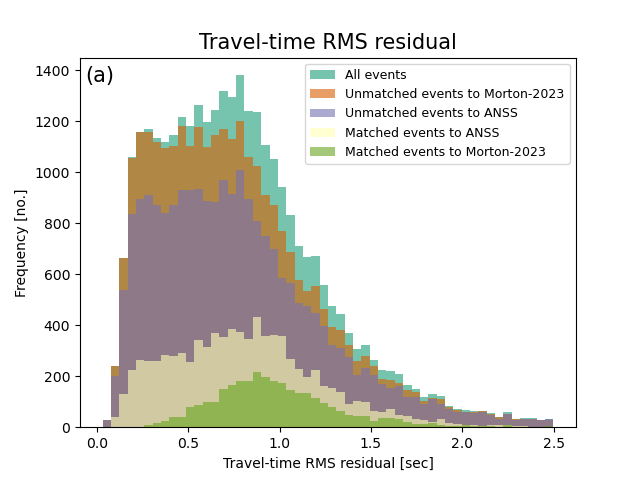
\includegraphics[width=0.48\textwidth]{figures/fig5_histograms/hist_rms_reloc_cog_ver3_p_4_s_4_rms_2_5.png}
  \hfill
  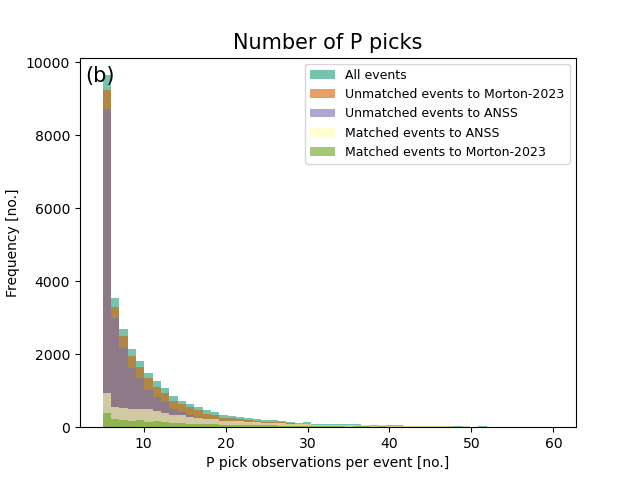
\includegraphics[width=0.48\textwidth]{figures/fig5_histograms/hist_p_picks_reloc_cog_ver3_p_4_s_4_rms_2_5.png}
  \vspace{0.5em}
  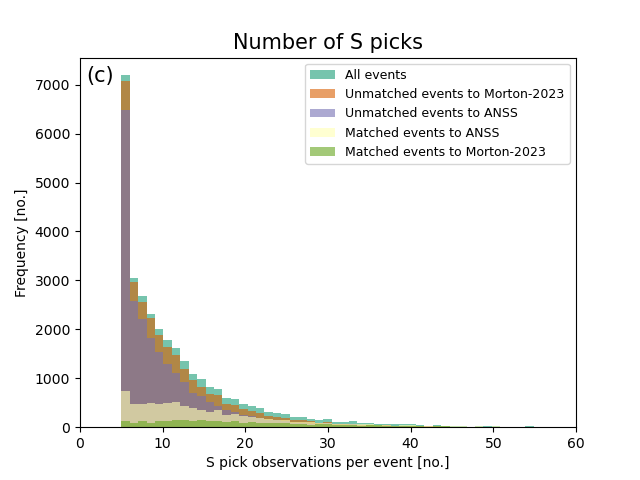
\includegraphics[width=0.48\textwidth]{figures/fig5_histograms/hist_s_picks_reloc_cog_ver3_p_4_s_4_rms_2_5.png}
  \hfill
  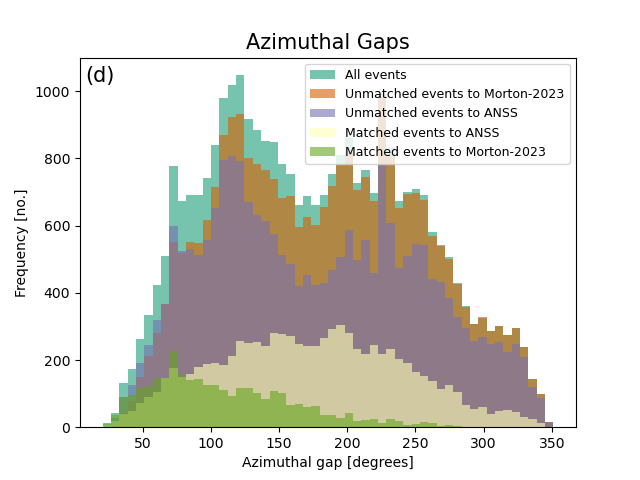
\includegraphics[width=0.48\textwidth]{figures/fig5_histograms/hist_gaps_reloc_cog_ver3_p_4_s_4_rms_2_5.png}
  \caption{
  {\bf Distributions of QC metrics for our catalog.} Panels show (a) RMS
  travel-time residual, (b) number of P picks, (c) number of S picks, and (d)
  azimuthal gap. }
  \label{fig:qc}
\end{figure*}

We required a minimum number of 5 P and 5 S picks to associate the
events.

\begin{figure}
    \centering
    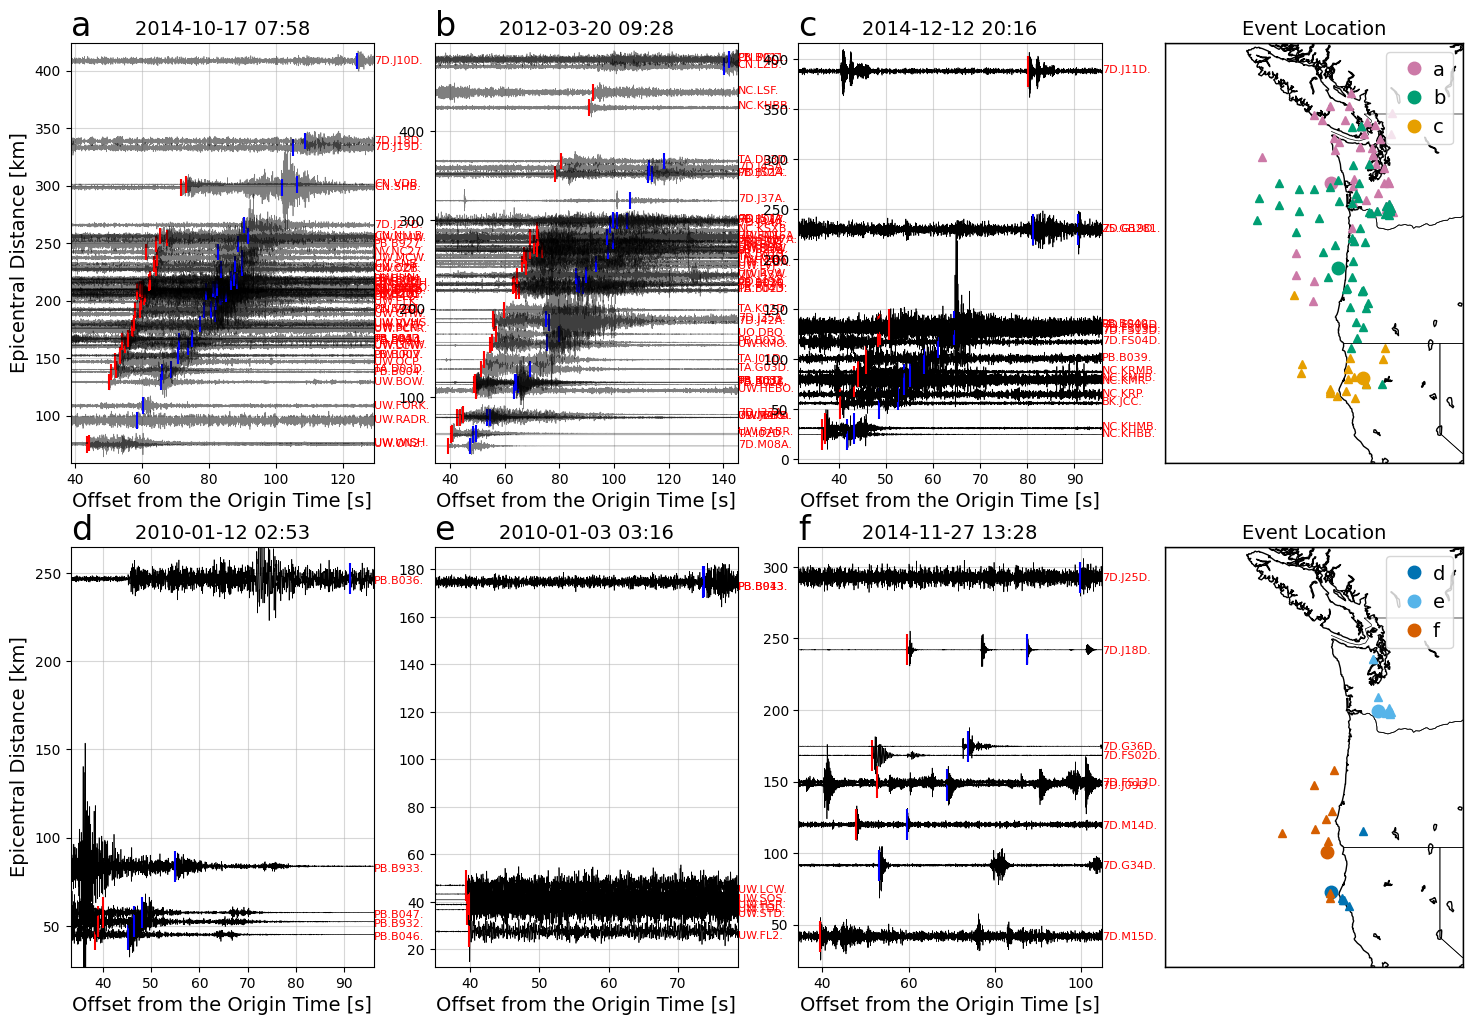
\includegraphics[width=\linewidth]{figures/fig3.png}
    \caption{Example of successful and unsuccessful picking and associated
    events}
    \label{fig:fig3}
\end{figure}

\subsection{Strategy to match with other
catalogs}\label{strategy-to-match-with-other-catalogs}

After the location, the events from all regions were merged into a
single catalog and matched with the catalogs from Morton et al.~2023 and
ANSS. The matched and unmatched events to these catalogs were mapped. In
addition, the waveforms of each event shallower than 5 km from the
merged catalog was plotted and manually checked to drop events that
didn't look like earthquakes. GraphDD was used for relocation (REF).

\section{Results}\label{sec:results}

Overall new statistics of the new catalog. How many picks, how many
associated, and a set of new events based on a few criteria (a
conservative, a medium conservative, a generous estimate).

Describe how many we matched with other catalogs. where do we match
best. Some possible differences are in the velocity models.

\begin{figure}
    \centering
    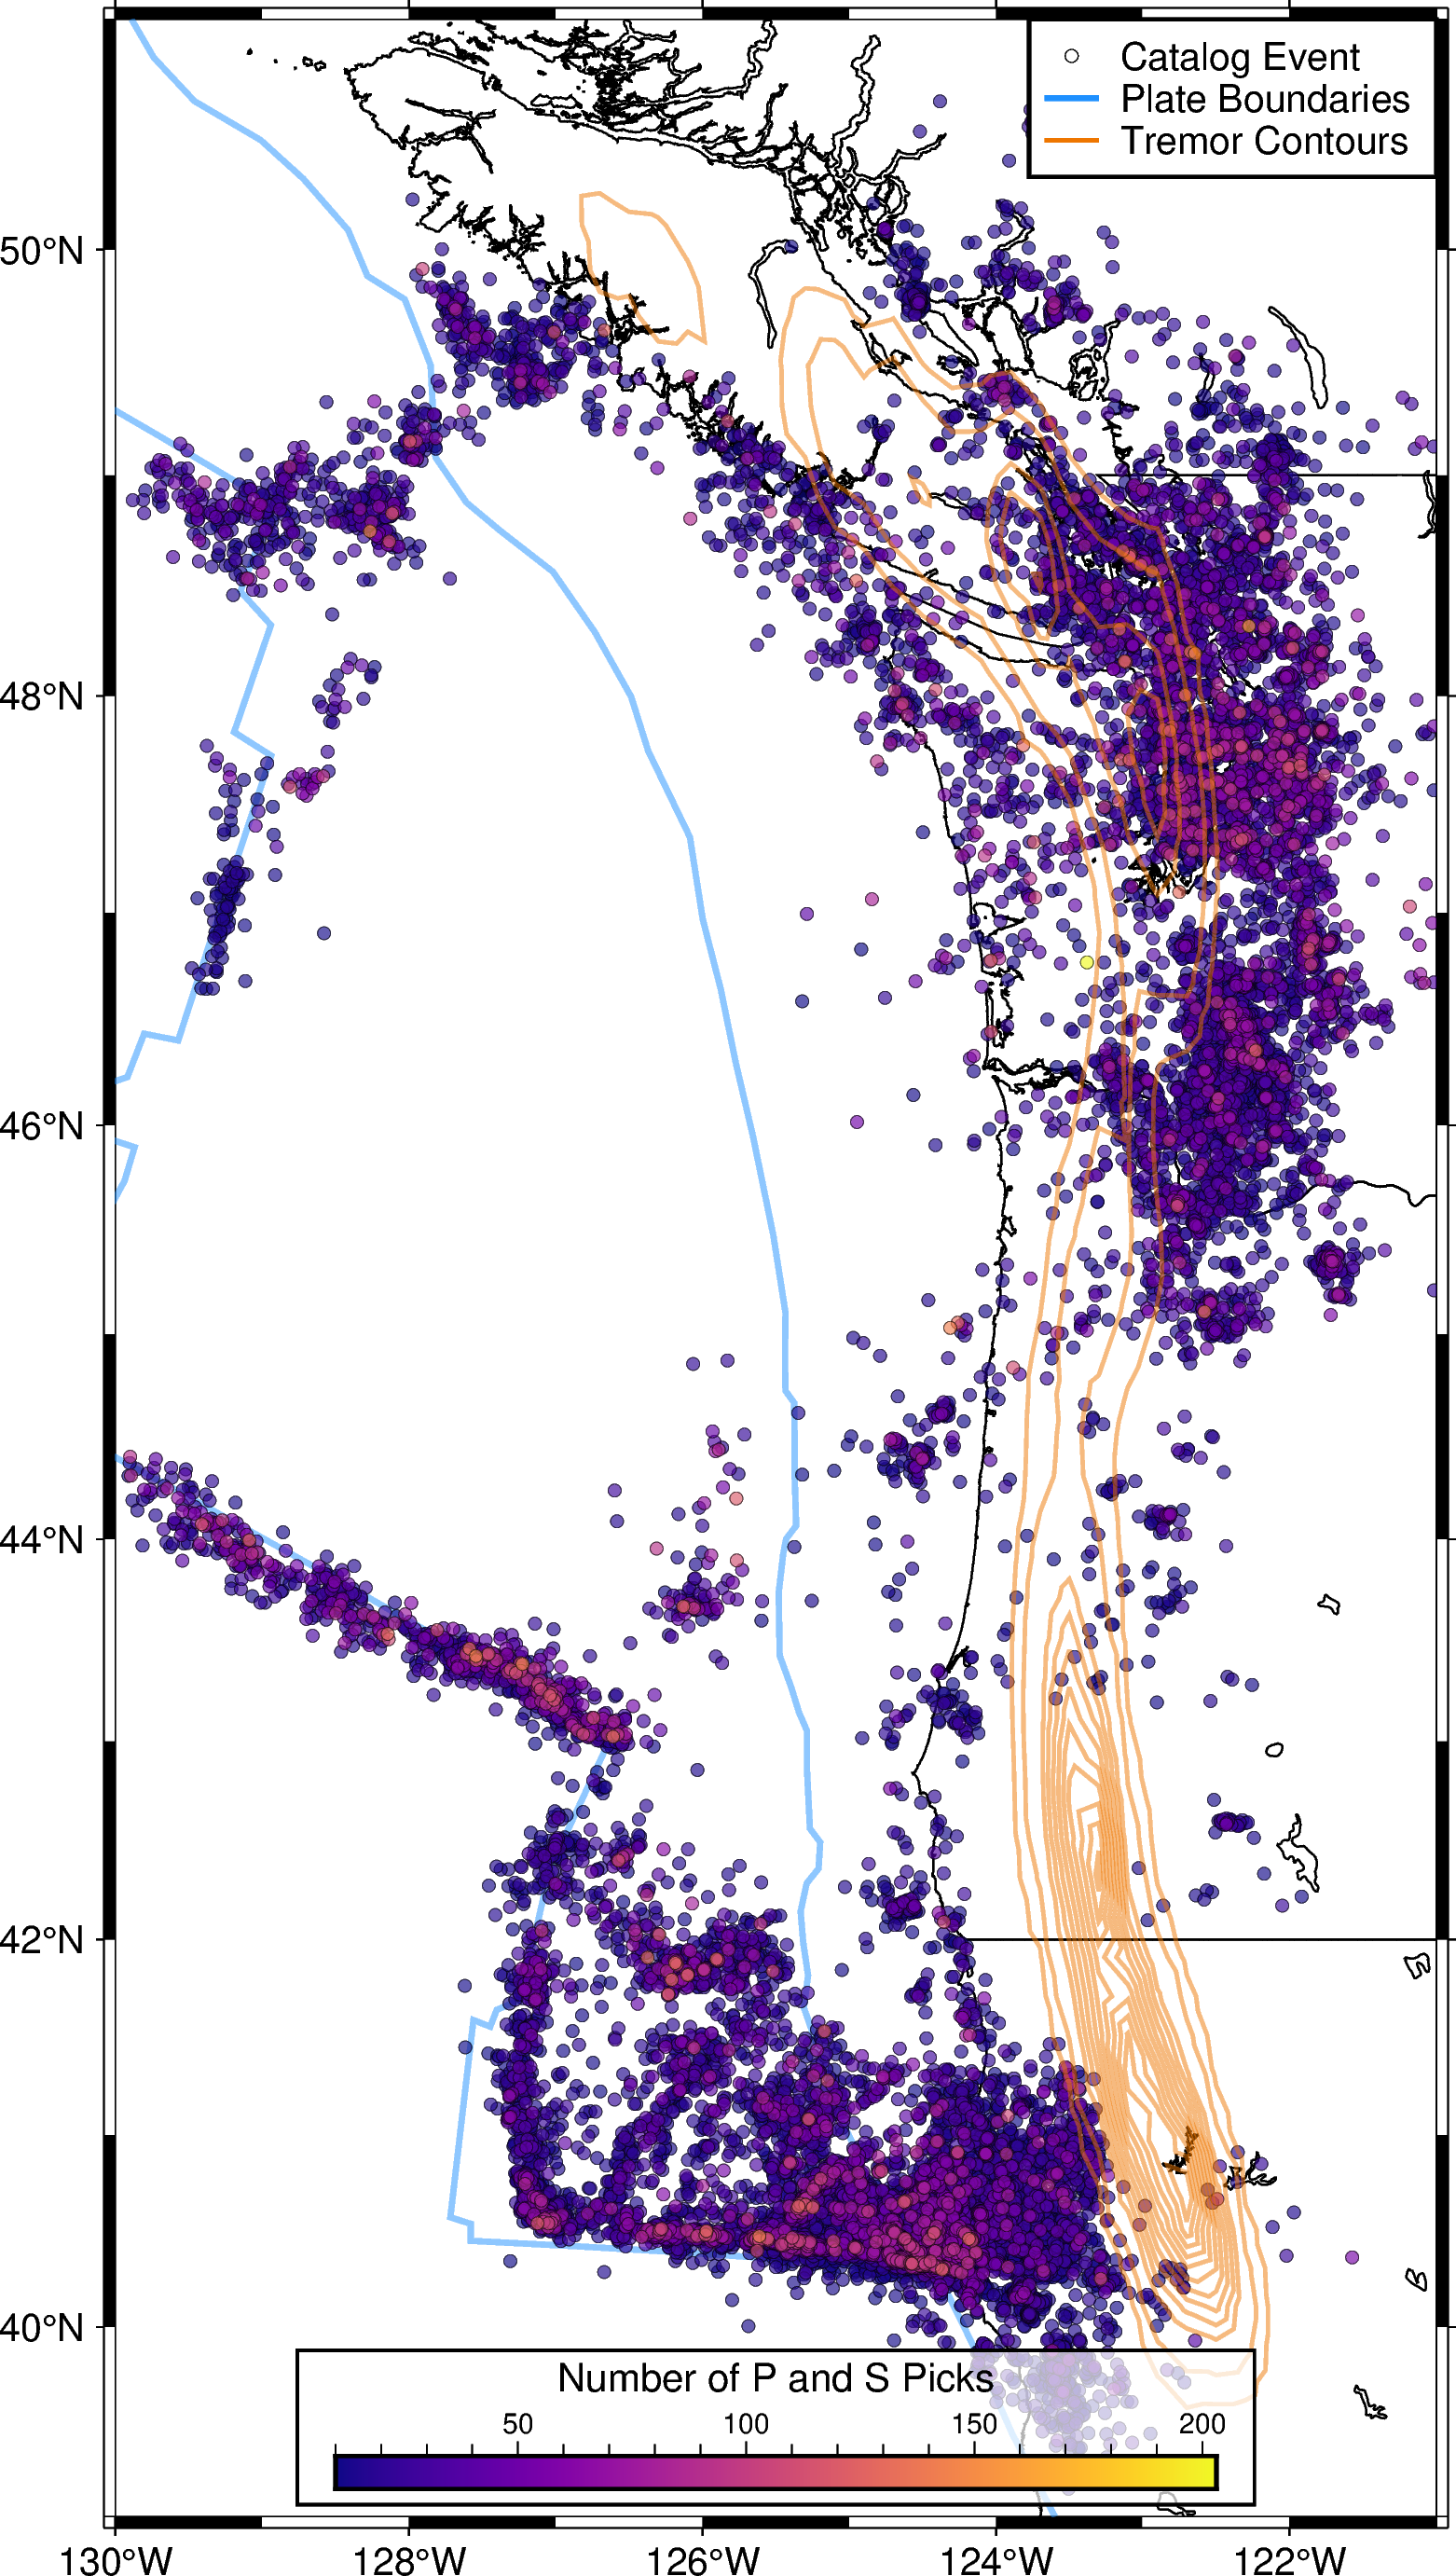
\includegraphics[height=\textheight]{figures/fig4_cc_no_relief_tremor_contours.png}
    \caption{{\bf New earthquake catalog}. (a) The new events that are matched
    with existing catalogs are shown in purple and linked to their matched
    events using a black line; the corresponding events from the ANSS catalogs
    are in blue, from the \citet{Morton23} catalog in green, and the remaining
    unmatched events are shown in green (Morton-2023) and yellow (ANSS). (b) New
    events were detected that met the quality control criteria and were
    color-coded by the number of picks.}
    \label{fig:fig4}
\end{figure}

\section{Discussion}\label{sec:disc}

We now analyze the novel seismicity and possible implications for
characterizing the tectonic processes across the multiple plate
boundaries.

\subsection{Endeavour and Nootka
Region}\label{endeavour-and-nootka-region}

\begin{figure}
    \centering
    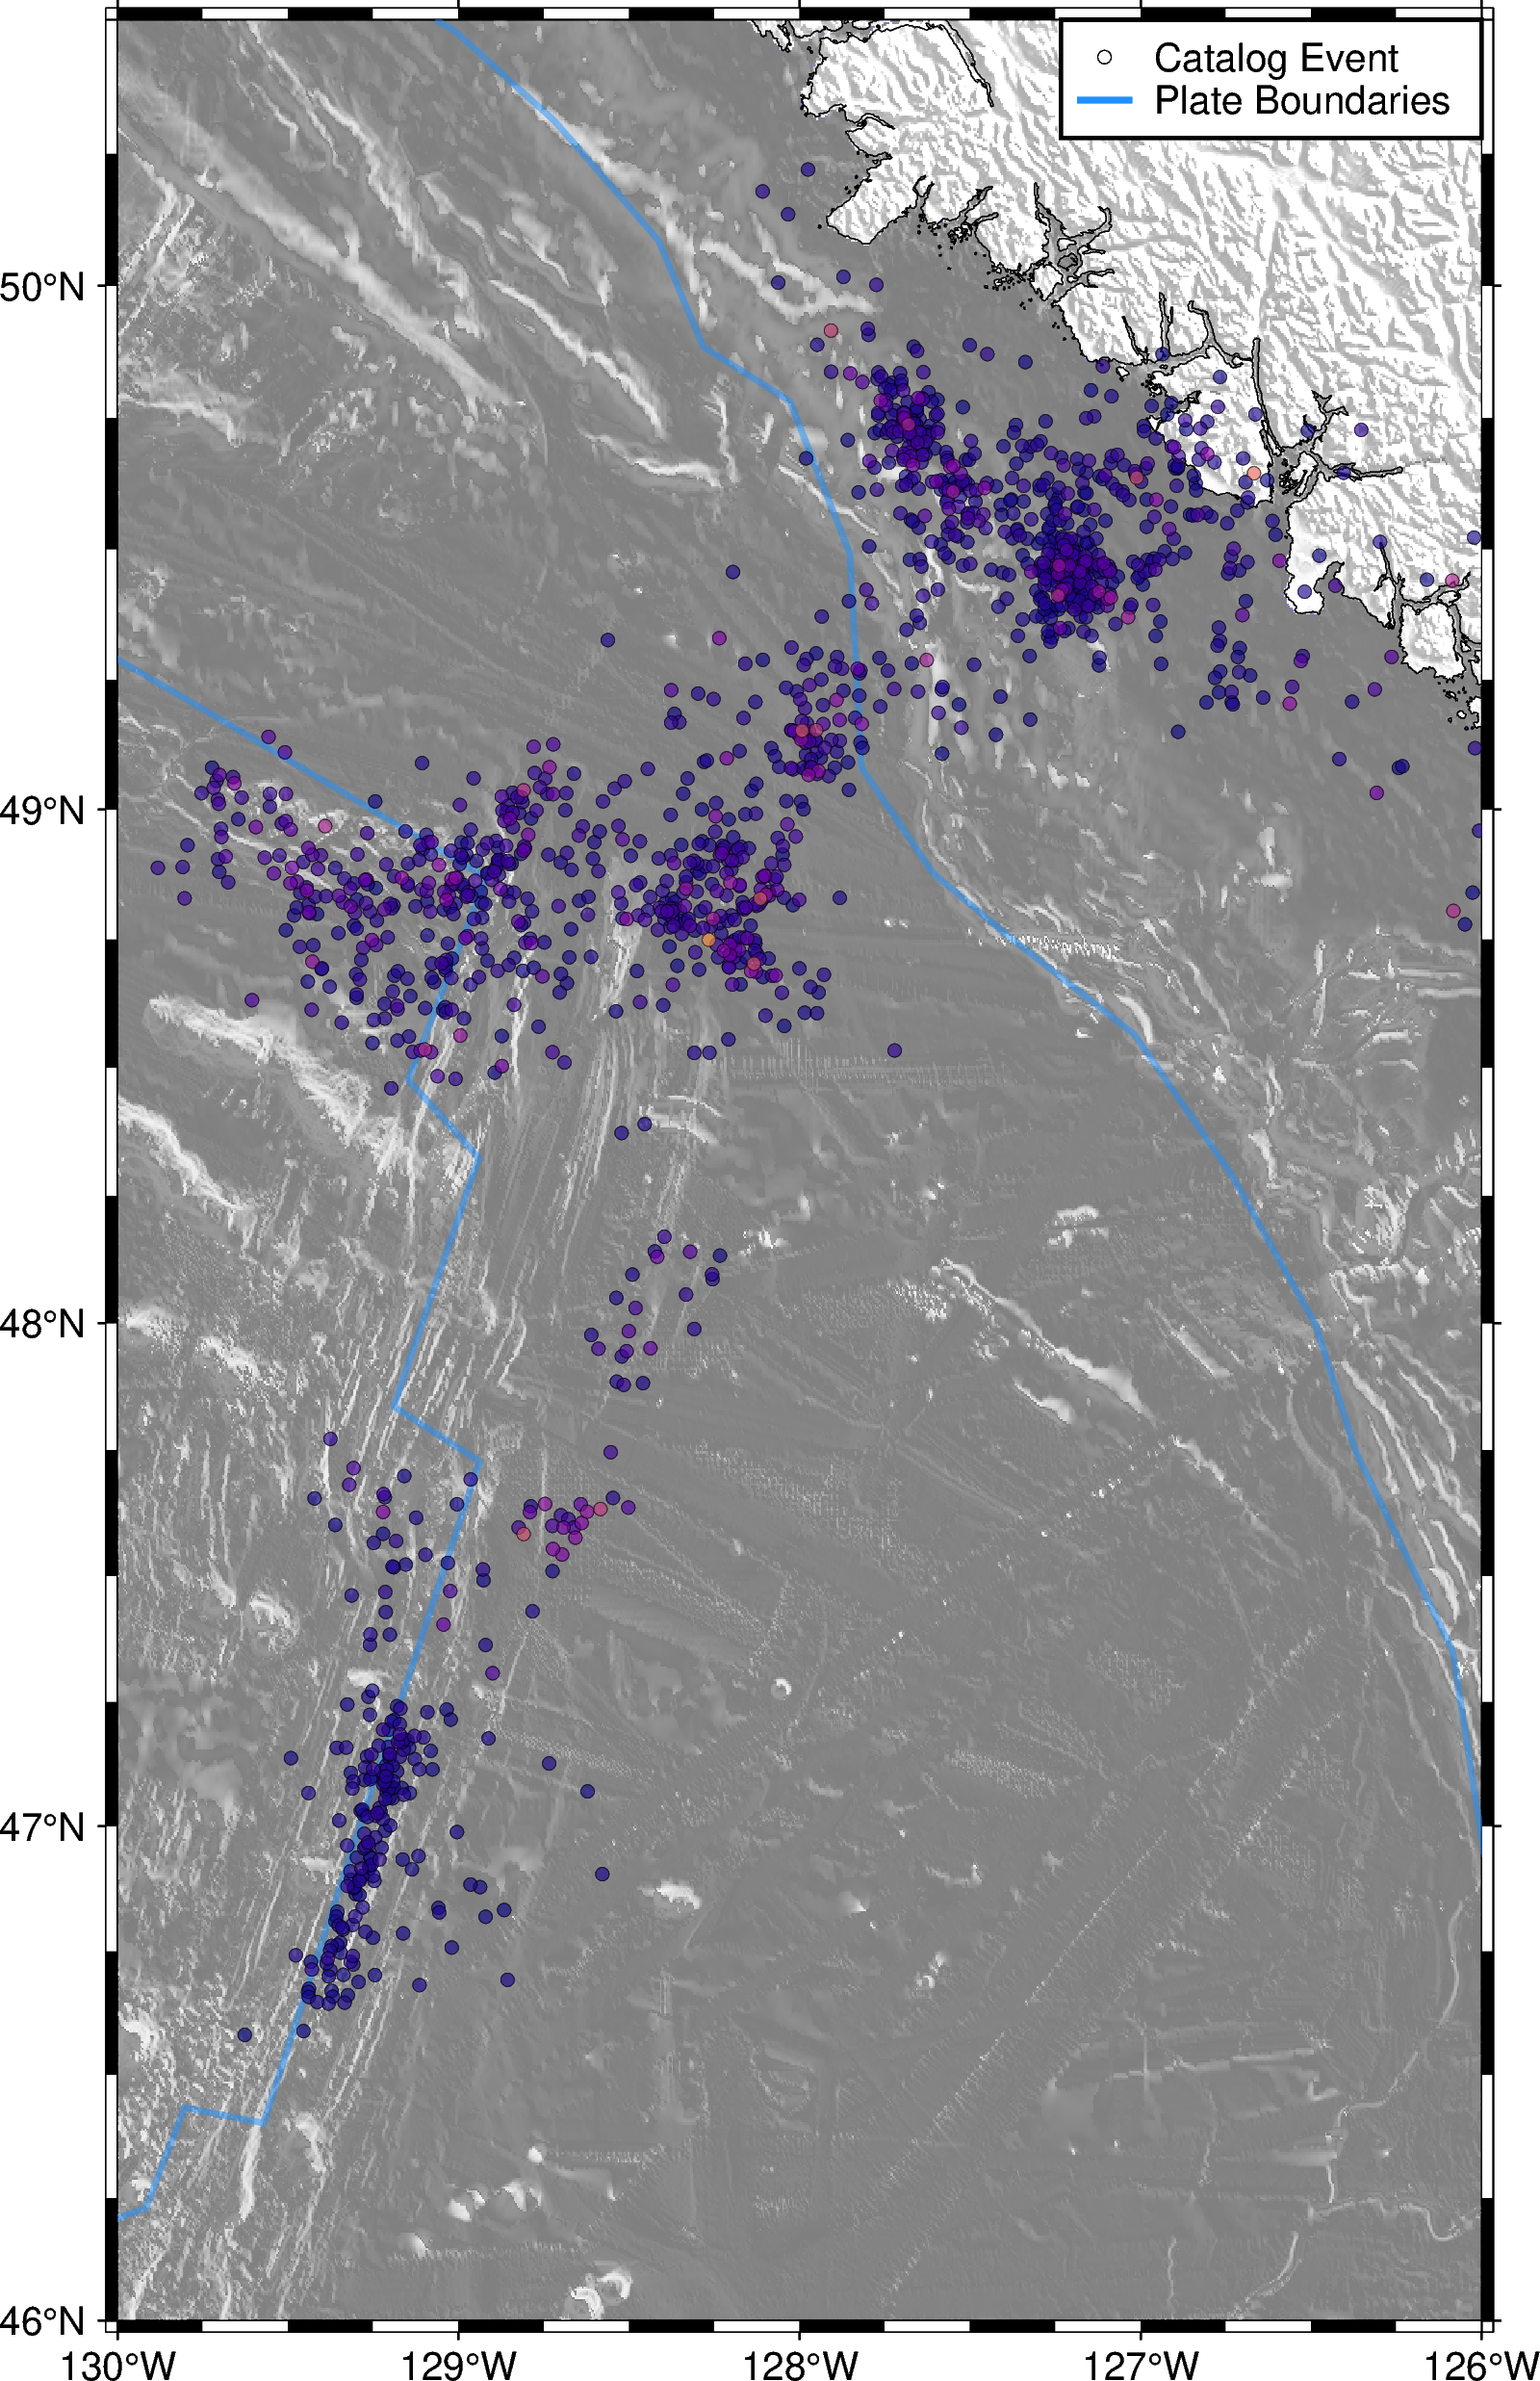
\includegraphics[width=0.8\linewidth]{figures/fig6.png}
    \caption{Earthquake Catalog in the Endeavor}
    \label{fig:fig6}
\end{figure}

The Nootka Fault Zone (NFZ) is the left-lateral, ridge-to-trench
transform boundary between the Juan de Fuca (JdF) and Explorer (ExP)
oceanic plates. It links the ridge-fault-fault triple junction at Middle
Valley on the spreading ridge to a fault-trench-trench triple junction
just seaward of Nootka Sound on Vancouver Island. First analysis of
seismic data by \citet{Hyndman79} showed a left-lateral fracture zone
with a relative motion of about 2--3 cm yr\(^{-1}\), accommodating the
faster subduction of the JdF plate south of the NFZ compared with the
ExP plate to the North. The structure of the NFZ is characterized by a
15-25 km wide fault visible in active seismic surveys \citep{Hyndman79},
and refined by recent precise earthquake relocation studies with two
almost vertical master strands---the Northern (NNF) and Southern (SNF)
Nootka faults---8--18 km apart, surrounded by several steep conjugate
faults and more diffuse lineations with several Riedel-style shear
\citep{Hutchinson19, hutchinson2023tectonic}, which explains well the
location of our newly found events at latitude 49N and longitude 138W.
\citet{Hutchinson19} determined the focal mechanisms of their catalog
and mainly found left-lateral strike-slip; normal faulting appears at
the SW (ridge-proximal) end, and thrust events emerge where the NFZ
dives beneath the continental slope NE of the deformation front. Our
catalog suggests a modest population on the ridge-proximal SW end that
future polarity measurements will help constrain as ridge-related.
Several large intraplate strike-slip events occurred in 2004, 2011, and
2014 \citep{Merrill22}. We note that the M6.6 2014 event on the Nootka
Sequence Fault (NSF) is well-documented in our catalog. Future
improvements to our catalog will enhance the depth resolution of our
newly discovered events and identify those related to the ``double
seismic zone'' identified in the recent tomography study by
\citet{Merrill22}.

\subsection{Mendicino and Blanco
Regions}\label{mendicino-and-blanco-regions}

short review of seismicity there and what this adds. context there is
the recent M6 earthquakes.

\subsection{Axial and Endeavour seamounts and
Nootka}\label{axial-and-endeavour-seamounts-and-nootka}

\subsection{Central Cascadia}\label{central-cascadia}

\subsection{Northern Cascadia}\label{northern-cascadia}

\subsection{Current limitations}\label{current-limitations}

Seismicity on the edge of of our box.

\section{Conclusion}\label{conclusion}

Thank all relevant parties and acknowledge funding sources, if any.

\section*{Data and Code Availability}\label{data-and-code-availability}
\addcontentsline{toc}{section}{Data and Code Availability}

All seismic data is available on the Earthscope Consortium and the
various networks used have digital identifiers objects,
\citep[C8][]{C8}, \citep[7D, 7A][]{7D}, \citep[CN][]{CN},
\citep[UW][]{UW}, \citep[UO][]{UO}, \citep[NC][]{NC}, \citep[BK][]{BK},
\citep[TA][]{TA}, \citep[OO][]{OO},, PB, \citep[X6][]{X6},
\citep[Z5][]{Z5}, \citep[X9][]{X9}. The software is available on GitHub
\url{https://github.com/Denolle-Lab/cascadia_obs_ensemble/} and on
zenodo (REF).

\section*{Competing interests}\label{competing-interests}
\addcontentsline{toc}{section}{Competing interests}

The authors declare no competing interests.


\bibliography{mybibfile}

\end{document}
